\chapter{Algoritmi otkrivanja društvenih zajednica}

Ključan dio u pronalasku društvenih zajednica u društvenim mrežama su algoritmi koji ih otkrivaju. Oni moraju biti pouzdani i učinkoviti, ali se i izvršavati u prihvatljivom vremenskom okviru. Algoritmi se testiraju na brojnim skupovima podataka uz prikladne evaluacijske mjere kako bi se zaključilo u kojim uvjetima koji algoritam daje najbolje rješenje. 

Grafove koji predstavljaju društvene zajednice teško je prikazati u ravnini ako teže stvarnim veličinama koje se kreću u tisućama čvorova, a često i mnogo više, što znači da se ne može iz ljuske perspektive odrediti kako bi dobar raspored zajednica izgledao. To znači da su algoritmi koji pronalaze društvene zajednice nenadzirani algoritmi koji sami, bez primjera za učenje i unaprijednog znanja o njima pokušavaju pronaći rješenje. U društvenim mrežama algoritmi koriste topološke karakteristike i specifičnosti koje posjeduju ovakvi tipovi mreža. 

Dvije važne tehnike na kojima se temelji većina algoritama su particioniranje i grupiranje. Particioniranje grafova je proces u kojem se graf dijeli na unaprijed određeni broj manjih komponenti pomoću određenog svojstva. Svojstvo koje se može iskoristiti je minimalni rez. Ono se koristi tako da se graf podijeli na dva ili više razdvojenih podgrafova, a veličina reza koja se pokušava minimizirati je broj bridova koje je potrebno ukloniti da bi to ostvarili. Potrebno je odrediti i svojstvo koje bi odredilo veličinu komponenti kao primjerice minimalan ukupan stupanj vrhova kako bi se dobila rješenja koja imaju smisla. Zbog takvih zahtjeva ovakav pristup najčešće nije prihvatljiv jer broj zajednica nije moguće unaprijed odrediti.
Grupiranje je proces u kojem se entitete koji imaju zajedničke karakteristike svrstava u iste grupe. Pronalaženje grupa može dati informacije o skrivenim značajkama, vezama i svojstvima članova te koliko su međusobno čvrsto povezani. U hijerarhijskom grupiranju stvara se hijerarhija među zajednicama. Proces se može odvijati na dva načina, aglomerativni ili divizivni. U aglomerativnom načinu se koristi pristup koji ide od dna prema vrhu te se određeni čvor dodaje drugim sličnim čvorovima te se koristi određeni kriterij sličnosti. U divizivnom načinu veće grupe dijele se na manje uz korištenje određene mjere koja govori koliko je dobra trenutačna podjela prema kojoj će se odrediti konačan rezultat.



\section{Girvan-Newmanov algoritam}

Veliko zanimanje i rast aktivnosti znanstvene zajednice u području društvenih mreža potaknuo je rad Girvana i Newmana iz 2002. godine \cite{girvan2002community} u kojem su predstavili novi algoritam koji se po njima i naziva. Dotad poznati algoritmi pokušavali su pronalaženje zajednica riješiti tako da bi provodili hijerarhijsko grupiranje. U početnom koraku kreće se od nepovezanog grafa te se za svaki par vrhova računa težina koja predstavlja koliko su vrhovi bliski. Tada se bridovi se dodaju jedan po jedan počevši od onih vrhova čija je bliskost najveća. Postoji više načina kako izračunati bliskost i temelje se na broju puteva između čvorova, npr. broj vršno nezavisnih putova ili bridno nezavisnih putova i slično. Takve definicije ipak u nekim slučajevima nisu uspješne i daju krive rezultate. Događa se da se vrhovi koji su na rubovima zajednice, povezani jednim bridom prema ostatku mreže izdvajaju iz zajednice kojoj pripadaju i ostaju potpuno izolirani od svih zajednica. Girvan-Newmanov algoritam pokušava suprotno, pronaći bridove koji što manje doprinose povezanosti unutar zajednica. 

Algoritam traži bridove koji povezuju zajednice te ih kroz iteracije uklanja i izolira zajednice. Za pronalazak bridova koristi se mjera različitosti, u ovom slučaju mjera bridne centralnosti. Njezina vrijednost računa se za svaki brid tako što se za sve parove vrhova odredi najkraći put te se svim bridovima koji se nalaze u tom putu dodaje vrijednost 1. Ako postoji $N$ najkraćih putova između vrhova onda se u svim putevima svakom bridu vrijednost povećava za $ \dfrac{1}{N} $. Bridna centralnost svakog vrha na početku je postavljena na 0. Postupak se ponavlja dok god postoji bridova u grafu. Izračunavanje bridne centralnosti je skupa operacija jer je potrebno za svaki par vrhova u svakoj iteraciji pronaći najkraći put te odrediti bridne centralnosti Mora se provoditi u svakom koraku jer se inače mogu dogoditi pogreške u koracima algoritma zato što se mreža prilagođava novom stanju nakon uklanjanja svakog brida. Takva situacija može se dogoditi ako su dvije zajednice povezane sa više bridova. Tada je prema algoritmu, sigurno da će barem jedan od tih bridova imati visoku bridnu centralnost te se zato nakon njegovog uklanjanja vrijednost mjere mora ponovno odrediti, a onda će jedan od preostalih bridova imati najvišu vrijednost. Moguće je uštedjeti nešto resursa tako što se bridna centralnost izračunava samo za one vrhova na koje je uklanjanje prethodnog brida imalo utjecaja. 

\bigskip
\begin{algorithm}
\caption{Girvan-Newmanov algoritam}
\begin{algorithmic}[1]
	\STATE izračunati mjeru različitosti za sve bridove u grafu
	\STATE ukloniti brid sa najvećom vrijednosti mjere različitosti
	\STATE za svaki brid izračunati mjeru različitosti nakon uklanjanja brida
	\STATE ponavljati korake 2 i 3 dok ima bridova u grafu
\end{algorithmic}
\end{algorithm}
\bigskip

Konačno rješenje algoritma određuje se tako što se u svakoj iteraciji računa modularnost za trenutnu podjelu grafa. Modularnost je mjera koja se koristi za procjenu jakosti veza unutar zajednice i jakosti veza među zajednicama. Njome je moguće izmjeriti koliko je određena podjela grafa kvalitetna. Ona podjela koja ima najvišu vrijednost na kraju algoritma uzima se kao rezultat. O modularnosti i ostalim mjerama mjerenju rezultata više će biti rečeno u poglavlju \ref{vrednovanja_i_rezultati} koje se bavi vrednovanjem rezultata algoritama.


Postupak traženja zajednica tijekom rada algoritma može se predstaviti dendogramom. Dendogram je prema strukturi stablo gdje su listovi pojedini vrhovi mreže. Prema vrhu stabla vrhovi se spajaju u zajednice te konačno u cijelu strukturu grafa. Vrhovi povezani na nižim razinama imaju snažnije međusobne veze. Rez kroz stablo na bilo kojoj razini daje skup zajednica koji u tom trenutku postoji. Gdje stablo odrezati određuju se pomoću modularnosti. Primjer je prikazan na slici \ref{fig:dendogram}.

\begin{figure}
	%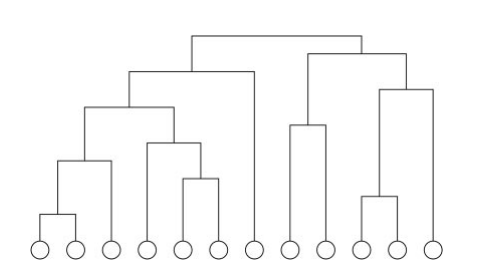
\includegraphics[width=\linewidth]{images/dendogram.png}
	\makebox[\textwidth][c]{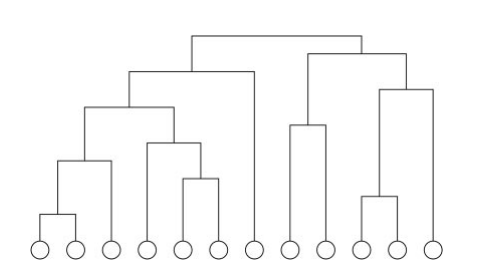
\includegraphics[width=0.8\textwidth]{images/dendogram.png}}
	\caption{Primjer hijerarhijskog stabla. Moguće je po koracima vidjeti kada je koji brid uklonjen iz mreže te kako su grupe nastale.}
	\label{fig:dendogram}
\end{figure}

Za graf od \textit{m} bridova i \textit{n} vrhova složenost algoritma u najgorem slučaju je $\mathcal{O}(m^{2}n)$. Potrebno je u svakom koraku algoritma ponovno izračunati mjeru različitosti što ima velik utjecaj na povećanje složenosti. U boljim slučajevima, kada se mreža nakon nekoliko iteracija razdvoji u nekoliko komponenti izvođenje algoritma znatno se ubrzava. U nekoliko slučajeva isprobana je strategija da se mjera različitosti izračuna jednom, na početku izvođenja algoritma, ali u radu \cite{girvan2002community} se pokazalo da takav postupak ne daje ispravna rješenja.

\pagebreak

\section{Louvain algoritam}

Algoritam osmišljen na sveučilištu u Louvainu stvoren je kako bi nadmašio dotad poznate algoritme u području otkrivanja zajednica. Objavljen je u radu \cite{blondel2008fast}, 2008. godine. Algoritam je testiran pronalaženjem zajednica u belgijskoj telefonskoj mreži od 2.6 milijuna korisnika te analiziranjem web grafa od 118 milijuna čvorova i više od milijardu bridova za koji je rješenje izračunao u 152 minute. Kapaciteti algoritma i testiranih mreža bili su ograničeni samo dostupnim kapacitetom računalnih resursa, a ne vremenom potrebnim za računanje. Algoritam se koristi heurističkom metodom koja se temelji na optimizacije modularnosti. 

Rad algoritma podijeljen je u dvije faze koje se ponavljaju kroz iteracije. U prvom koraku, za graf od \textit{N} čvorova, svaki čvor pripada zajednici u kojoj je samo on član što znači da u početku postoji onoliko zajednica koliko graf ima čvorova. Tada se za svaki čvor \textit{i} promatraju njegovi susjedi \textit{j} te se računa promjena modularnosti koja bi se dogodila ako se čvor \textit{i} premjesti u zajednicu čvora \textit{j}. Čvor \textit{i} se premješta u zajednicu za koju je promjena maksimalna i pozitivna, odnosno modularnost raste. Ako je nema rasta promatrani čvor ostaje u dodijeljenoj zajednici. Proces se ponavlja slijedno dok god postoje poboljšanja. Moguće je da se svi čvorovi razmatraju kroz nekoliko iteracija. Kada se u iteraciji ne dogodi niti jedno poboljšanje algoritam završava prvu fazu. U radu \cite{blondel2008fast} pokazalo se kako redoslijed čvorova nema značajnijeg utjecaja na rezultat, ali se može uštedjeti na vremenu izračunavanja. Dio učinkovitosti algoritma proizlazi iz jednostavnog računanja promjene modularnosti tijekom premještanja čvora \textit{i} u grupu \textit{C} koja se dobiva prema sljedećem izrazu: 
\begin{equation}
	\Delta Q =  \bigg[ \frac{\sum_{in} + k_{i,in}}{2m} - \bigg( \dfrac{\sum_{tot} + k_{i} }{2m} \bigg)^{2} \bigg] 
	- 
	\bigg[ \dfrac{\sum_{in}}{2m} - \big( \dfrac{\sum_{tot}}{2m} \big)^{2} - \bigg( \dfrac{k_{i}}{2m} \bigg)^{2} \bigg] .
\end{equation}
\bigskip
$\sum_{in}$ predstavlja sumu težina bridova, \textit{C}, $\sum_{tot}$ je suma težina bridova koji su povezani sa čvorovima u zajednici \textit{C}, $k_{i}$ je suma težina bridova koji su incidentni sa čvorom \textit{i}. $k_{i,in}$ je suma težina bridova koji povezuju čvor \textit{i} sa zajednicom \textit{C} i \textit{m} je broj bridova u cijeloj mreži. U primjeni se promjena modularnosti računa tako što se čvor \textit{i} premješta iz trenutne zajednice u susjedne te se promatra kako se vrijednosti ponašaju.

\bigskip
\begin{algorithm}
	\caption{Louvain algoritam}
	\begin{algorithmic}[1]
		\REQUIRE graf \textit{G}
		\REPEAT 
		\STATE svaki čvor grafa $G$ dodijeliti u vlastitu zajednicu
		\WHILE{postoje čvorovi koji se premještaju}
		\FORALL{čvor $n$ grafa $G$}
		\STATE postaviti čvor u susjednu zajednicu uključujući i trenutnu tako da se rast modularnosti maksimizira
		\ENDFOR
		\ENDWHILE
		\IF{nova modularnost veća od prethodne} 
		\STATE {graf $G$ postaje novi graf sa čvorovima koje čine prethodno dobivene zajednice} 
		\ELSE \STATE{kraj} 
		\ENDIF
		\UNTIL{}
	\end{algorithmic}
\end{algorithm}
\bigskip

Druga faza algoritma sastoji se od građenja nove mreže čiji čvorovi postaju zajednice koje su pronađene tijekom prve faze. Kako bi se dobio cjelovit graf potrebno je nove čvorove povezati bridovima. Brid se dodaje tako da spaja zajednice čiji su čvorovi bili susjedni te mu je težina suma težina tih bridova. Ako je brid bio unutar zajednice predstavlja se petljom koju je moguće izostaviti. U početnom koraku za graf koji nema određene težine bridova, težine se mogu postaviti na 1. Kada druga faza završi ponavlja se prva faza na novonastalu mrežu. Ako se promotri rad algoritma te činjenicu da je u početku svaki čvor jedna zajednica, onda se može zaključiti da se broj zajednica kroz iteracije smanjuje te je resursno najzahtjevnija prva iteracija. Faze se ponavljaju dokle god ima promjena u strukturi zajednica te modularnost ne postigne maksimum. Može se primijetiti da se kroz proces algoritma prirodno uključio pojam hijerarhije kada se manje zajednice spajaju u veće. Visina hijerarhije ovisi o broju iteracija algoritma te je uobičajeno manji broj.

Algoritam je jednostavan, intuitivan i jednostavan za implementaciju te radi nenadzirano. Složenosti je $\mathcal{O}(n \cdot log{}n)$. Zbog pohlepne optimizacije, jednostavnog izračuna promjene modularnosti i naglog rasta broj zajednica brzo se izvršava što se dodatno ističe u mrežama su rijetke i koje imaju čvrste strukture zajednica. Postoji problem koji se događa zbog modularnosti koja ima problem u prepoznavanju manjih zajednica što se naziva rezolucijski limit. Njegov utjecaj ublažen je time što algoritam u početnom koraku kreće od situacije gdje je svaki čvor u svojoj zajednici te je vjerojatnost da će dvije različite zajednice biti spojene tako da se čvorovi premještaju jedan po jedan vrlo niska. Ako zajednice pokažu veliku bliskost mogu se spojiti kasnije nakon što se čvorovi u njima združe. Takvo ponašanje ističe se u slučaju klika koje konačno budu u jednoj zajednici, ali su razdvojene u početnim prolazima što znači da je moguće dobiti uvid u rješenja međukoraka algoritma te se krajnjem korisniku tako može pružiti uvid u promatranje zajednica na određenoj rezoluciji, odnosno hijerarhijskoj razini.


\section{Surprise algoritam}

Surprise algoritam uvodi novu mjeru kvalitete podjele zajednica u mreži. U radovima \cite{blondel2008fast} i \cite{gamermann2022algorithm} prikazano je kako modularnost ima određenih nedostataka. Događa se problem s rezolucijom te se manje zajednice združuju s većima pri čemu može doći do situacije da povezanost čvorova unutar zajednice postaje slaba. Modularnost također posjeduje mnogo sličnih lokalnih maksimuma što znatno otežava pronalaženje globalnog. Moguća je i situacija u kojoj se za strukturno vrlo različite podjele zajednica dobivaju slične vrijednosti modularnosti. Mjera koja bi trebala riješiti navedene probleme naziva se surprise. Predstavljena je u radu \cite{aldecoa2010jerarca} kao mjera za procjenu kvalitete pronađenih zajednica algoritama hijerarijskog grupiranja. U mnogim radovima mjera je korištena za ocjenjivanje rezultata raznih algoritama, ali u radu \cite{gamermann2022algorithm} je iskorištena kao dio algoritma.


U grafu sa \textit{K} čvorova i \textit{n} bridova podijeljenih u $N_{c}$ zajednica takvih da je $l$ bridova mreže povezuje vrhove iste zajednice surprise mjera definira se na sljedeći način:

\begin{equation}
	S = - ln \sum_{j = l}^{min(M,m)} \frac{ {M \choose j} {F-m \choose n-j} }{ {F \choose n}}.
\end{equation}
Mjera je hipergeometrijska distribucija gdje $F$ predstavlja maksimalan broj mogućih bridova u mreži, $F = \frac{K(K-1)}{2}$ dok je $M$ maksimalan moguć broj bridova unutar $N_{c}$ zajednica gdje je broj čvorova unutar zajednice $i$, $c_{i}$. $M$ se računa prema sljedećem izrazu:
\begin{equation}
	M = \sum_{i=1}^{N_{c}} \frac{c_{i}(c_{i}-1)}{2}.
\end{equation} 
Surprise mjeru može se zamisliti kao mjerenje koliko je malo vjerojatno, iznenađujuće, pronaći zajednicu sa $l$ bridova unutar nje kao u promatranoj mreži. Postupak se može promatrati kao posuda sa $F$ loptica gdje svaka loptica predstavlja jedan od mogućih bridova unutar mreže, gdje ih je $M$ crveno koji predstavljaju moguće bridove unutar zajednice, a $F-M$ ih je plavih koji predstavljaju bridove između različitih zajednica. Iz posude se izvlači $n$ loptica koje predstavljaju stvaran broj bridova u grafu. Suma s desne strane jednadžbe je vjerojatnost izvlačenja barem $l$ crvenih loptica. Obično vrijedi da je $M << F$ te vjerojatnost izvlačenja crvene loptice može biti niska.

Surprise algoritam detekcije zajednica sličan je Louvain algoritmu. U početnom koraku mreža se podijeli u onoliko zajednica koliko ima čvorova. Tada algoritam pokušava premještanjem čvorova pronaći takvu raspodjelu koja će maksimizirati vrijednost surprise mjere. Razlika u odnosu na Louvain algoritam je što se premještanje čvorova može obavljati na tri načina. Dvije zajednice mogu biti spojene u jednu, jedan čvor se može premjestiti iz jedne u drugu zajednicu ili se čvor može izdvojiti u novu grupu. Druge dvije operacije mogu se pokrenuti rekurzivno za svaku zajednicu što algoritmu daje dodatnu snagu. Time je moguće otkriti manje podgrupe unutar zajednice te ih potencijalno izdvojiti u novu zajednicu ili pridružiti nekoj od postojećih. Operacije također pomažu algoritmu u izbjegavanju lokalnih maksimuma.

Algoritam je pohlepan što znači da prati svako poboljšanje vrijednosti surprise mjere koje pronađe sve dok ih više ne može naći. Istraživanja u radu \cite{gamermann2022algorithm} su pokazala da neke druge strategije u biranju smjera u kojem će surprise mjere rasti nisu pokazala bolje rezultate od pohlepne strategije dok su bile računalno zahtjevnije, no mogu se koristiti u završnim koracima algoritma kada razlike u rastu mjere postaju male.


\begin{algorithm}
	\caption{Surprise algoritam}
	\begin{algorithmic}[1]
		\REQUIRE mreža \textit{G}
		\WHILE{postoje promjene u mreži} 
			\FOR{svaka zajednica u mreži} 
				\FOR{svaki čvor u zajednici} 
					\FOR{svaki susjed čvora} 
						\IF{zajednica susjeda različita od trenutne zajednice} 
							\STATE {pokušati spojiti zajednice ili izmijenti čvorove između njih} 
						\ENDIF
					\ENDFOR
				\ENDFOR 
				\WHILE{postoje promjene} 
					\STATE{izdvojiti čvor iz zajednice} 
				\ENDWHILE
				\WHILE{postoje promjene} 
					\STATE{izdvojiti podzajednicu iz zajednice} 
				\ENDWHILE
				\WHILE{postoje promjene} 
					 \FOR{svaku drugu zajednicu u mreži} 
					 	\STATE {pokušati premjestiti podzajednicu u drugu zajednicu} 
					 \ENDFOR
				\ENDWHILE				
			\ENDFOR
		\ENDWHILE
	\end{algorithmic}
\end{algorithm}

Algoritam iterira kroz zajednice dok god se događaju promjene u strukturi zajednica. U svakoj zajednici prolazi kroz sve čvorove te ih pokušava pridružiti susjednima pojedinačno ili kao čitavu zajednicu. Potom pokušava iz svake zajednice izdvojiti čvor, izdvojiti podzajednicu ili je premjestiti u drugu zajednicu. Postojanje promjene znači da je određena operacija podigla vrijednost surprise mjere za novu raspodjelu.

Postoji velik broj kombinacija kako se čvorovi mogu podijeliti u zajednice te ih nije moguće sve provjeriti. Važno je promotriti kako se konfiguracija zajednica ponaša u situacijama kada su lokalni maksimumi slične vrijednosti te koliko su blizu globalnog. U radu \cite{gamermann2022algorithm} je pokazano da surprise algoritam ne pati od problema degeneracije ako je lokalni maksimum blizu globalnog što znači da i u slučajevima kada maksimum surprise mjere nije postignut konfiguracija mreže je reprezentativna što za modularnost nije vrijedilo. Ipak ne postoji garancija da će globalni maksimum biti pronađen, ali algoritam uz surprise mjeru trebao bi dati bolje rješenje u odnosu na onaj s modularnosti.



\section{Leiden algoritam}

Leiden algoritam osmišljen kako bi ispravio nedostatke Louvain algoritma. Lovain algoritam može kao konačan rezultat pronaći slabo povezane zajednice u situacijama gdje su one i iznad i ispod ranije spomenutog problema s rezolucijskom granicom. Algoritam može premjestiti čvor koji je predstavljao most između komponenti trenutne zajednice u drugu zajednicu dok ostali čvorovi ostaju u zajednici i ne premještaju se u neku od prikladnijih u tom trenutku. Događanje navedenog primjera izbjegava se u slučajevima kada je zajednica iznutra čvrsto povezana. Primjer opisane situacije nalazi se na slici \ref{fig:bridge-node}. U a) dijelu čvorovi od 0 do 6 su u istoj zajednici te kada se čvor 0 premjesti zajednica prestaje biti povezana. Tada bi se dvije manje zajednice trebale moći izdvojiti u zasebne. Problem nastaje kada je zajednica lokalno optimalna te algoritam provodi drugu fazu u kojoj agregira zajednicu u jedan čvor što je najgori slučaj. Tada više nije moguće raditi premještanja unutarnjih čvorova te zajednica ostaje nepovezana osim ako se slučajno dogodi da se poveže sa nekom zajednicom koja će poslužiti kao novi most.

\begin{figure}
	%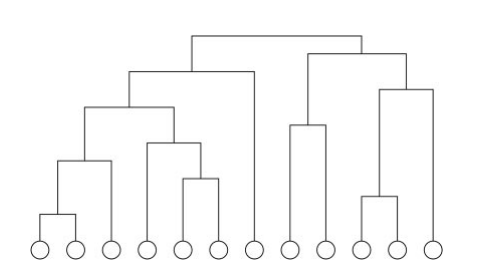
\includegraphics[width=\linewidth]{images/dendogram.png}
	\makebox[\textwidth][c]{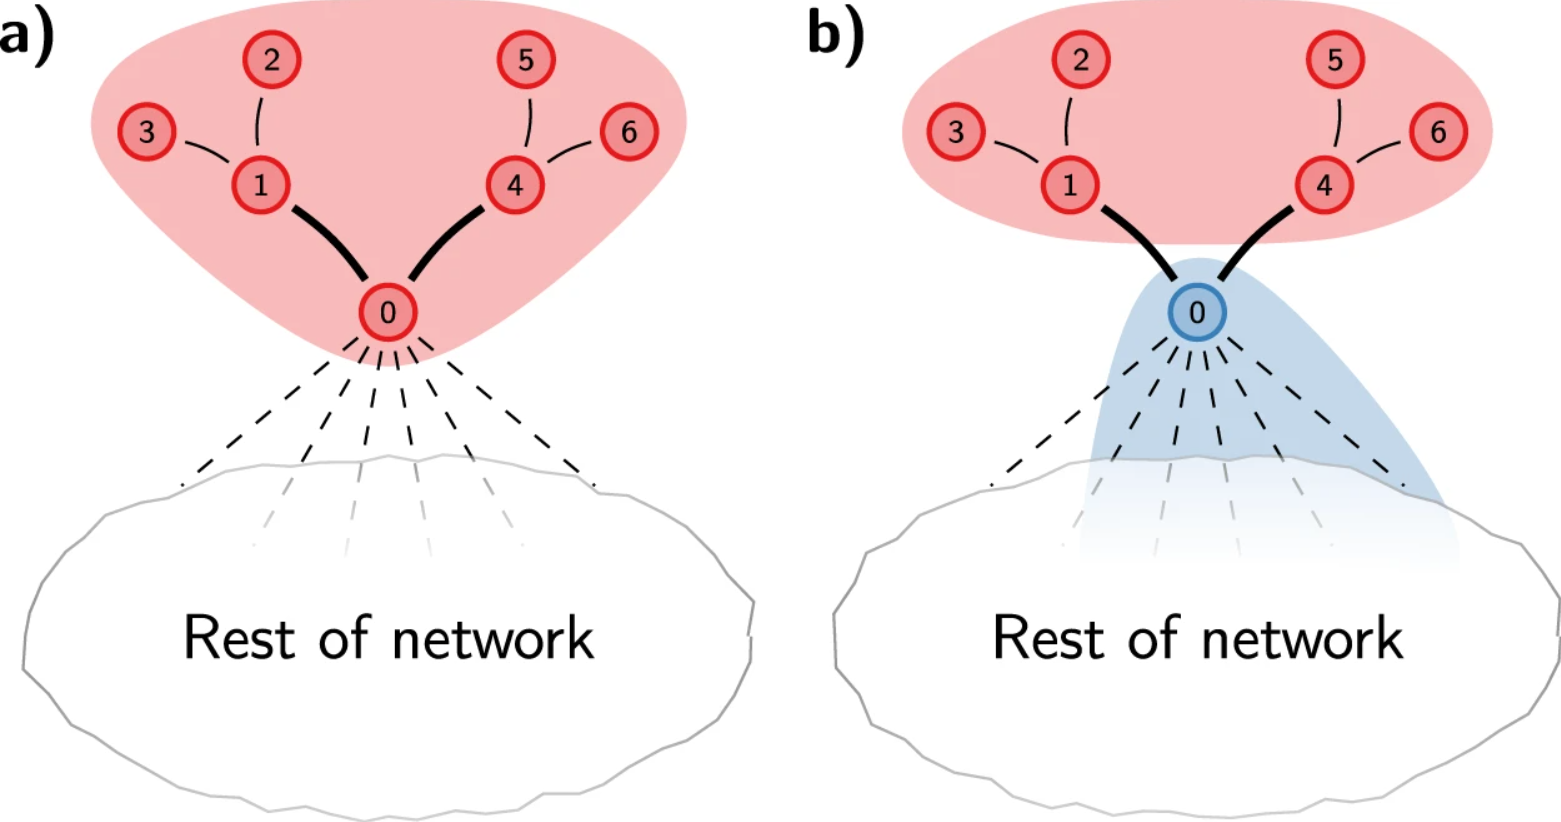
\includegraphics[width=0.7\textwidth]{images/bridge-node.png}}
	\caption{Primjer premještanja čvora iz zajednice u kojoj je predstavljao most između unutarnjih komponenti iz rada \cite{traag2019louvain}.}
	\label{fig:bridge-node}
\end{figure}


Leiden algoritam predstavljen je u radu \cite{traag2019louvain} 2019. godine te pokušava ispraviti nedostatke Louvaina korištenjem raznih, već poznatih strategija prilikom premještanja čvorova. Algoritam pametnog premještanja čvorova predstavljen je u radu \cite{waltman2013smart}. Leiden koristi ideju o ubrzavanju premještanja lokalnih iz rada \cite{ozaki2016simple} te ideju o premještanje čvora u zajednicu slučajno izabranog susjednog čvora iz rada \cite{traag2015faster}. Algoritam kao i Louvain radi premještanja na temelju optimizacije modularnosti.

Leiden algoritam sastoji se od tri faze: lokalno premještanje čvorova, pročišćavanje zajednica i agregacija mreže temeljena na pročišćenim zajednicama. U Louvain algoritmu agregacija zajednica u nove čvorove stvara se na temelju trenutnih zajednica. Leiden algoritam pokušava pročistiti pronađene zajednice prije koraka agregacije. Tim korakom zajednica se može podijeliti u podzajednice koje će bolje predstavljati strukturu mreže. Pročišćene zajednice se tada agregiraju u čvorove za iduću iteraciju algoritma. Podjela zajednica ostaje ista kakva je bila prije faze pročišćavanja, kao u Louvain algoritmu. Implementacijom faze pročišćavanja dobiva se bolja šansa da će algoritam pronaći zajednice visoke kvalitete i povezanosti.

\begin{figure}
	%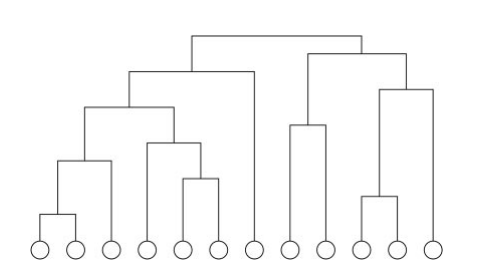
\includegraphics[width=\linewidth]{images/dendogram.png}
	\makebox[\textwidth][c]{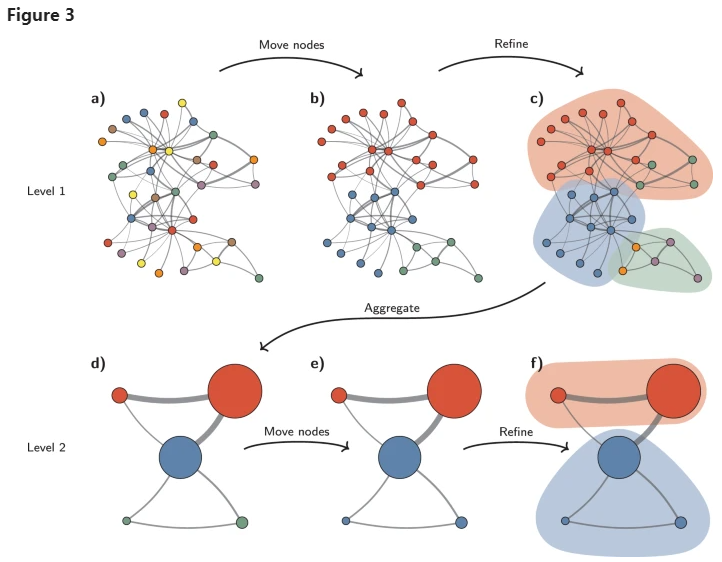
\includegraphics[width=0.8\textwidth]{images/leiden.png}}
	\caption{Ilustracija dvije iteracije Leiden algoritma iz rada \cite{traag2019louvain}. U a) dijelu čvorovi se podijele u zasebne zajednice te se na slici b) spajaju u zajednice. Na c) slici provodi se proces pročišćavanja zajednica i proces kreće u novu iteraciju.}
	\label{fig:leiden}
\end{figure}

Pročišćavanje se provodi na sličan način kao i prva faza algoritma, ali na razini zajednice. Svakom čvoru se dodijeli vlastita zajednica te se čvorovi lokalno spajaju sa drugima unutar zajednice ako su njihove veze dovoljno jake. Tijekom procesa pročišćavanja čvorovi se ne premještaju nužno pohlepno nego mogu biti dodani bilo kojoj zajednici za koju vrijednost funkcije kvalitete raste. Zajednica u koju će se čvor dodati odabire se slučajno, tako da je veća što je veći rast funkcije kvalitete. Razina slučajnosti ovisi o parametru $\theta > 0$. Slučajnost doprinosi istraživanju prostora zajednica i omogućava izlaženje iz potencijalnih lokalnih maksimuma. Isključivanje premještanja koja bi negativno utjecala na funkciju kvalitete nisu dozvoljena jer bi previše usporavala algoritam na velikim mrežama. 

%Nakon faze pročišćavanja zajednica će vrlo često biti podijeljena, ali to ne mora nužno biti tako. 

Još jedna razlika u odnosu na Louvain algoritam događa se u procesu lokalnog premještanja čvorova. Leiden algoritam koristi implementaciju brzog premještanja. Algoritam posjećuje čvorove dok god postoje promjene u funkciji kvalitete. U ovakvom pristupu posjećuju se samo oni čvorovi kojima se dogodila promjena u susjedstvu za razliku od Louvaina koji u svakoj iteraciji obilazi sve čvorove. Proces započinje tako da se u red dodaju svi čvorovi mreže slučajnim poretkom. Tada se uzima prvi čvor te se provjerava raste li funkcija kvalitete premještanjem u neku zajednicu. Ako se čvor premjesti, na kraj reda dodaju se svi susjedi čvora koji ne pripadaju novoj zajednici, a nisu već u redu. Proces se nastavlja dokle god red nije prazan. Korištenjem brzog premještanja prva iteracija je ista kao u Louvain algoritmu i obilaze se svi čvorovi, ali se u kasnijim iteracijama posjećuju samo oni čvorovi na koje promjene zaista utječu čime Leiden algoritam postaje značajno efikasniji.


\begin{algorithm}
	\caption{Leiden algoritam}
	\begin{algorithmic}[1]
		\REQUIRE mreža G
		\REPEAT 
			\STATE{lokalno premještanje čvorova}
			 \IF{svaka zajednica se sastoji od samo jednog čvora} 
			 	\STATE {\textbf{break}} 
			 \ELSE
			 	\STATE pročistiti zajednice
			 	\STATE agregirati mrežu na temelji pročišćenih zajednica
			 	\STATE zadržati određeni raspored zajednica 
			 \ENDIF
		\UNTIL		
	\end{algorithmic}
\end{algorithm}



\section{Walktrap algoritam}
Walktrap algoritam predstavlja novu mjeru kojom računa sličnosti između čvorova i zajednica. Mjera se temelji na slučajnim šetnjama kroz mrežu koje imaju dobra svojstva u smislu računalne složenosti i otkrivanja strukture zajednica. Algoritam koristi definiciju zajednice koja kaže kako su grafovi društvenih mreža globalno rijetki, ali lokalno gusti. Gusti dijelovi nazivaju se zajednice koje su čvrsto povezane s nekoliko veza prema ostatku mreže. Ideja algoritma temelji se tako što bi slučajne šetnje kroz graf trebale ostati zarobljene unutar gustih dijelova odnosno zajednica. Pomoću njih definiraju se mjere kojima se mogu mjeriti strukturalne sličnosti između čvorova i između zajednica. Dobiveni rezultati mogu se prikazati u hijerarhijskom obliku dendograma. Algoritam je predstavljen u radu \cite{pons2005computing}.

Proces slučajne šetnje kroz graf \textit{G} odvija se tako što slučajni šetač prelazi iz jednog čvora u drugi koji je izabran slučajno i uniformno u odnosu na ostale susjedne čvorove. Niz čvorova koji se posjećuju može se predstaviti Markovljevim lancem gdje su stanja vrhovi grafova. Vjerojatnost prijelaza iz čvora $i$ u $j$ u svakom koraku je $ P_{i,j} = \frac{A_{i,j}}{d(i)} $, gdje je $A_{i,j}$ element u matrici susjedstva koji određuje jesu li čvorovi susjedni i iznosi 0 ako nisu ili 1 ako jesu, a $d(i)$ je stupanj čvora $i$. Isto se može zapisati kao matrica prijelaza slučajne šetnje $P$ te se računa pomoću izraza $P = D^{-1}A$ gdje je $D$ dijagonalna matrica stupnjeva vrhova, a $A$ matrica susjedstva. Proces slučajne šetnje odvija se potenciranjem matrice $P$. Vjerojatnost prijelaza iz čvora $i$ u $j$ kroz $t$ koraka je $(P^{t})_{i,j}$. 

Vjerojatnost zadovoljava dva svojstva karakteristična za proces slučajne šetnje. Prvo se odnosi vjerojatnost da se šetač nađe u čvoru $j$ ovisi samo o njegovom stupnju kada duljina šetnje $t$ teži prema beskonačnosti:
\begin{equation} \label{svojstvo1}
	\forall i, \lim_{t\to+\infty} P_{i,j}^{t} = \frac{d(j)}{\sum_{k}d(k)},
\end{equation}
gdje $\sum_{k}d(k)$ predstavlja sumu vrhova svih čvorova u grafu.
Drugo svojstvo kaže kako je vjerojatnost prelaska iz čvora $i$ u $j$ i iz $j$ u $i$ tijekom slučajne šetnje $t$ ima omjer koji ovisi samo u stupnjevima čvorova: 
\begin{equation} \label{svojstvo2}
	\forall i, \forall j, d(i) P_{i,j}^{t} = d(j) P_{i,j}^{t}.
\end{equation}
Dokazi su navedeni u radu \cite{pons2005computing}.

Mjera udaljenosti $r$ osmišljena je kako bi mjerila sličnost između čvorova u grafu. Udaljenost mora biti velika ako čvorovi pripadaju različitim zajednicama i mala ako su unutar iste. Računa se pomoću informacija dobivenih iz slučajnih šetnji. Za slučajnu šetnju duljine $t$ kojom se dobiva informacija o vjerojatnosti prijelaza iz čvora $i$ u $j$ bitno je da duljina $t$ dovoljno duga kako bi se prikupilo dovoljno informacija o topologiji mreže, ali duljina ne smije biti prevelika kako bi se izbjeglo prethodno navedeno svojstvo u izrazu \ref{svojstvo1} te vjerojatnost ne bi ovisila samo o stupnju čvora u koji se ide. Svaka vjerojatnost $P_{i,j}^{t}$ nosi određene informacije o čvorovima $i$ i $j$, a svojstvo \ref{svojstvo2} govori kako vjerojatnosti $P_{i,j}^{t}$ i $P_{j,i}^{t}$ nose istu količinu informacije što se može iskoristiti u definiranju potrebne mjere. Kako bi se mjera ispravno koristila potrebno je istaknuti nekoliko činjenica. Ako je iznos vjerojatnost $P_{i,j}^{t}$ visok ne mora nužno značiti da su čvorovi $i$ i $j$ unutar iste zajednice. Na vjerojatnost $P_{i,j}^{t}$ utječe stupanj čvora $d(j)$ zato što se vjerojatnost da će slučajna šetnja u njemu završiti povećava što je stupanj veći. Konačno ako su dva čvora u istoj zajednici trebali bi ostatak mreže promatrati na isti način što znači da ako su $i$ i $j$ u istoj zajednici vrijedi $\forall k, P_{i,k}^{t} \approx P_{j,k}^{t}$, gdje je $k$ bilo koji čvor u mreži. Mjera udaljenosti između dva čvora definira se sljedećim izrazom:
\begin{equation}
	r_{i,j} = \sqrt{\sum_{k=1}^{n} \frac{(P_{ik}^{t} - P_{jk}^{t})^{2}}{d(k)}}
\end{equation}

Na sličan način moguće je generalizirati udaljenost između čvorova na udaljenost između zajednica. Slučajna šetnja počinje iz jednog od slučajno, uniformno odabranih čvorova zajednice. Vjerojatnost $P^{t}_{C,j}$ šetnje iz zajednice $C$ do čvora $j$ se računa:
\begin{equation}
	P^{t}_{C,j} = \frac{1}{|C|} \sum_{i \in C} P^{t}_{i,j},
\end{equation}
gdje je $|C|$ broj čvorova unutar promatrane zajednice. Mjera udaljenosti između dvije zajednice tada se definira na sljedeći način pri čemu vrijede ista načela kao i u definiciji udaljenosti između čvorova:
\begin{equation}
	r_{C_{1}C_{2}} = \sqrt{\sum_{k=1}^{n} \frac{(P_{ik}^{t} - P_{jk}^{t})^{2}} {d(k)}}
\end{equation}


\begin{algorithm}
	\caption{Walktrap algoritam}
	\begin{algorithmic}[1]
		\REQUIRE mreža G
		\STATE podijeliti graf u $n$ zajednica
		\FOR{$k$ od 1 do $n-1$ } 
			\STATE izabrati zajednice $C_{1}$ i $C_{2}$ prema kriteriju udaljenosti između zajednica
			\STATE spojiti odabrane zajednice u novu $C_{3} = C_{1} \cup C_{1}$, dodati je grafu i izbaciti stare
			\STATE izračunati promjenu u udaljenosti između zajednica
		\ENDFOR		
	\end{algorithmic}
\end{algorithm}

Algoritam započinje podjelom svih vrhova u zasebne zajednice. Kroz $n$-1 koraka prema kriteriju udaljenosti spaja po dvije zajednice i dodaje ih u mrežu. Nakon dodavanja nove zajednice u mrežu računaju se nove udaljenosti među zajednicama, ali samo onima koji su u susjedstvu nove. Konačna struktura može se prikazati dendogramom u kojem se može vidjeti u kojem koraku su određene zajednice spojene.

Središnji dio algoritma predstavlja izračun kvalitete strukture zajednica. Kako bi se smanjila kompleksnost algoritma moguće je spajati samo susjedne zajednice. Zajednice koje će se spojiti biraju se prema Wardovoj metodi minimalne varijance. U svakom od $k$ koraka spajaju se dvije zajednice koje minimiziraju srednju vrijednost kvadratne udaljenosti između svakog čvora i njegove zajednice.
\begin{equation}
	\sigma_{k} = \frac{1}{n} \sum_{C \in P_{k}} \sum_{i \in C} r_{iC}^{2}
\end{equation}
Pristup je pohlepan i pokušava riješiti problem tako da uzima najbolje rješenju u koraku $k$. Problem je NP-težak i poznat je iz drugih algoritama grupiranja, npr. K-Medijana u radu \cite{de2003approximation}, koji su ga pokušali iskoristiti, ali aproksimacije su bile eksponencijalne složenosti. Aproksimacijska promjena varijance računa se tako da se za svaki par susjednih zajednica izračuna promjena $ \Delta \sigma (C_{1} C_{2})$ koja bi se dogodila kada bi se zajednice $C_{1}$ i $C_{2}$ spojile u novu zajednicu $C_{3}$. Rezultat ovisi samo o čvorovima zajednica $C_{1}$ i $C_{2}$. Računa se prema sljedećem izrazu:
\begin{equation}
	\Delta \sigma (C_{1} C_{2}) = \frac{1}{n} \bigg( \sum_{i \in C_{3}}r_{iC_{3}}^{2} - \sum_{i \in C_{1}}r_{iC_{1}}^{2} - \sum_{i \in C_{2}}r_{iC_{2}}^{2} \bigg)
\end{equation}
Konačno spajaju se dvije zajednice za koje je $\Delta \sigma$ najmanje vrijednosti.
